%----------------------------------------------------------------------------------------
%	PACKAGES AND OTHER DOCUMENT CONFIGURATIONS
%----------------------------------------------------------------------------------------

\documentclass[a0,portrait]{a0poster}
\usepackage{subfigure}
\usepackage{multicol} % This is so we can have multiple columns of text side-by-side
\usepackage[svgnames]{xcolor} % Specify colors by their 'svgnames', for a full list of all colors available see here: http://www.latextemplates.com/svgnames-colors
\usepackage{times} % Use the times font
\usepackage{graphicx} % Required for including images
\usepackage{booktabs} % Top and bottom rules for table
\usepackage[font=small,labelfont=bf]{caption} % Required for specifying captions to tables and figures
\usepackage{amsfonts, amsmath, amsthm, amssymb} % For math fonts, symbols and environments
\usepackage{wrapfig} % Allows wrapping text around tables and figures
\usepackage[export]{adjustbox}
\columnsep=100pt % This is the amount of white space between the columns in the poster
\columnseprule=3pt % This is the thickness of the black line between the columns in the poster
\graphicspath{{figures/}} % Location of the graphics files
\begin{document}
%----------------------------------------------------------------------------------------
%	POSTER HEADER 
%----------------------------------------------------------------------------------------
\begin{minipage}[t]{0.75\linewidth}
\VeryHuge \color{HoGentAccent1} \textbf{The migration process and advantages of Windows Server 2019} \color{Black}\\ % Title
\huge \textbf{Du Four Jens, Verschuere Glenn, Stroobants Ludwig}\\[0.5cm] % Author(s)
\huge Hogeschool Gent, Valentin Vaerwyckweg 1, 9000 Gent\\[0.4cm] % University/organization
\Large \texttt{jens.dufour.y2321@student.hogent.be} \\
\end{minipage}
\begin{minipage}[t]{0.25\linewidth}

\includegraphics[width=13cm,right]{figures/HOGENT_Logo_Pos_rgb.png} 
\end{minipage}
\vspace{1cm} % A bit of extra whitespace between the header and poster content
\begin{multicols}{2} % This is how many columns your poster will be broken into, a portrait poster is generally split into 2 columns
%----------------------------------------------------------------------------------------
%	ABSTRACT
%----------------------------------------------------------------------------------------
\color{HoGentAccent1} % Navy color for the abstract
\begin{abstract}
    This research covers the topic of Windows Server 2019, the different versions, and the advantages it has to its precursor Windows Server 2016.
	Windows Server is one of the most well established enterprise operating systems in the world. 
    This makes keeping it up-to-date in the fast paced world of information technologies crucial. 
    Thanks to the abundance of new features that come with every new version looking into the migration to the latest version is truely important.
    This bachelor's thesis will look into how the migration process from Windows Server 2016 to Windows Server 2019 would work.
    This while summerizing the advantages and possible disadvantages of this process. 
    First the migration of a typical Microsoft service, a Domain Controller, will be done.
    Afterwards an SAP environment, as described by delaware, will be migrated.
    To continue, A comparison will be made between the different available base container images and how these enhancements, as well as the new Windows base container image, can be leveraged.
    Finally, the further development of Windows Server over the years to come will be analysed.
    In the end, this research paper will advise for a migration to the latest version of the operating system.
\end{abstract}
%----------------------------------------------------------------------------------------
%	INTRODUCTION
%----------------------------------------------------------------------------------------
\color{HoGentAccent1} 
\section*{Introduction}
\color{black}
Windows Server is a well-known operating system among IT professionals. 
With major organizations all around the globe, like Infosys, that have implemented some form of the operating system in their infrastructure.
One of the tasks that often needs to be performed, is keeping applications up-to-date. 
However, it is not often described how to migrate the entire operating system to a newer version.  
This does not mean that frequent updates are not important for both the addition of new features as well as the improvement of security, as this is becoming one of the big concerns of this century. 
This bachelor's thesis will go in-depth about the advantages and disadvantages of migrating to the latest version of Windows Server.
In specific, this bachelor's thesis look at the migration from Windows Server 2016 to Windows Server 2019, with as an optional requirement the migration of a SAP environment, as this is applicable to the business environment of the originator, delaware.
The key purpose is to find a procedure that is efficient, minimizes possible downtime and is applicable not only to the originator, delaware, but also to other organizations that find them self in the same situation and want to migrate their infrastructure to the latest version of the operating system.
%----------------------------------------------------------------------------------------
%	GEOLOGY
%----------------------------------------------------------------------------------------
\color{Black} % DarkSlateGray color for the rest of the content
\color{HoGentAccent1} 
\section*{Experiment}
\color{black}
After the state of the art about the new features of Windows Server 2019, the migration was performed.
The proof of concept environment that was used is based on the Modern Desktop Deployment and Management Lab Kit provided by Microsoft. 
In this environment a Domain Controller was migrated using the in-place upgrade and side-by-side migration method using Windows Server 2016 as the starting point.
Afterwards, the migration of an SAP solution was done, this to show the additional research that is required to migrate a third-party software solution to the latest version of the operating system. 
\begin{center}\vspace{0.1cm}
    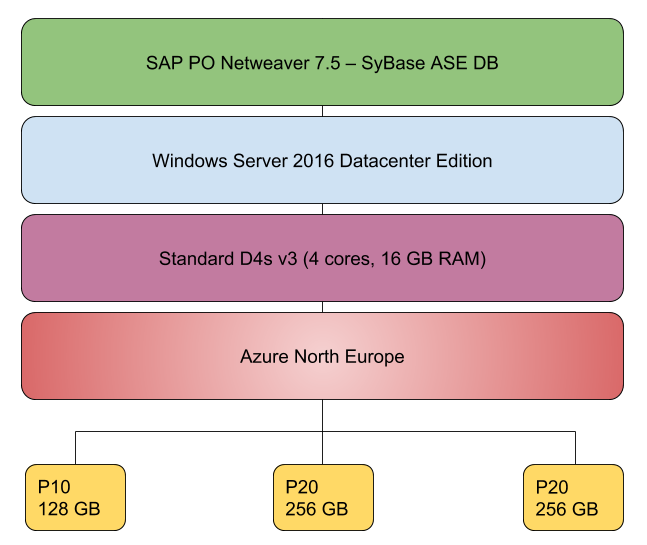
\includegraphics[width=\linewidth]{../bachproef/img/Methodologie/SAP_PO}
    \captionof{figure}{\color{HoGentAccent5} Infrastructure of the SAP environment}
\end{center}\vspace{0.1cm}
%\vfill\null
%\columnbreak
Finally, the advantages and disadvantages of the base container images that come with Windows Server 2019 were discussed.
At first, the Windows, Server Core and Nano Server were analysed in terms of size.
\begin{center}\vspace{0.1cm}
    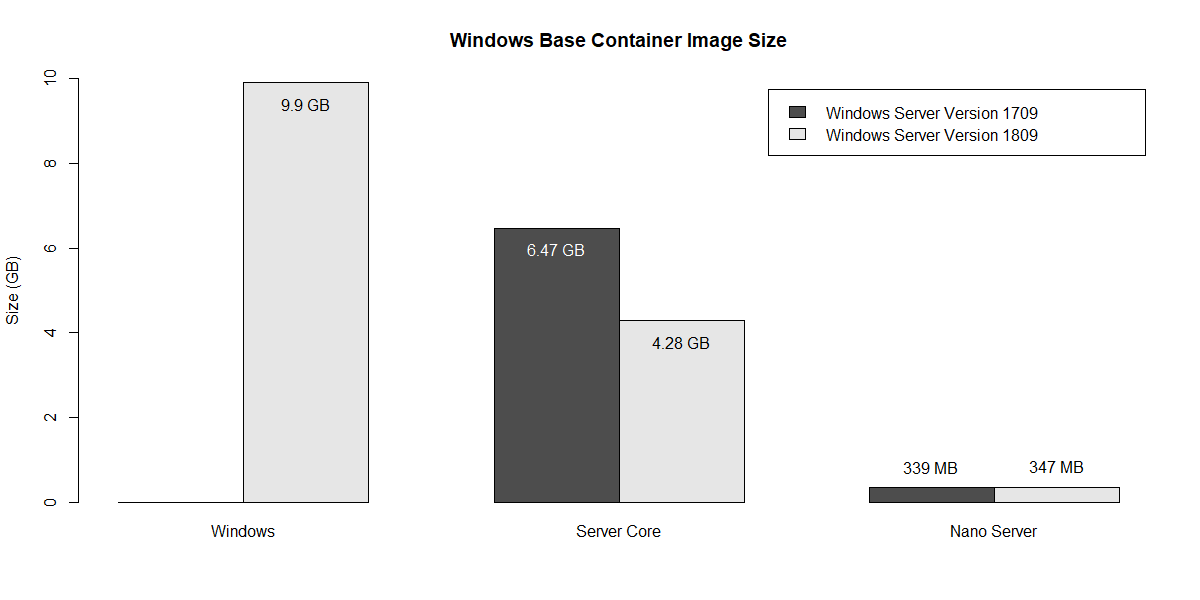
\includegraphics[width=\linewidth]{../bachproef/img/Methodologie/Containers0}
    \captionof{figure}{\color{HoGentAccent5} Comparison of the Windows base container image size}
\end{center}
Afterwards, a comparison of the performance was made. 
This was done using 'BenchmarkDotNet', a .NET library made for benchmarking.
\begin{center}
    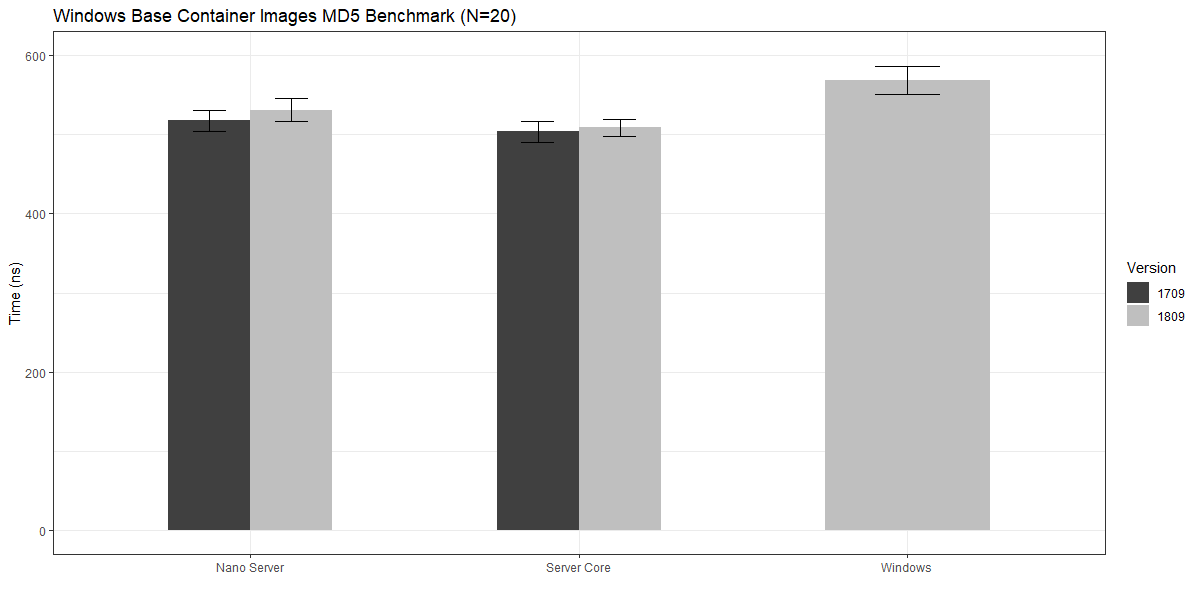
\includegraphics[width=\linewidth]{../bachproef/img/Methodologie/Containers1}
    \captionof{figure}{\color{HoGentAccent5} Base Container Image MD5 benchmark (N=20)}
\end{center}
%----------------------------------------------------------------------------------------
%	CONCLUSION
%----------------------------------------------------------------------------------------
\color{HoGentAccent1} 
\section*{Conclusion}
\color{black}
The conclusion of this bachelor's thesis is that a migration to Windows Server 2019 is achievable.
The latest version of the OS offers a smooth and manageable experience through the advancements made in the four key themes of Windows Server 2019. 
The extended support till 2029 makes it an ideal choice to future-proof any organization. 
While a migration to Windows Server 2019 in an environment with a third-party application requires additional research, it was attainable for a SAP environment. 
The migration from Windows Server 2016 to Windows Server 2019 is also feasible for any organization running an EOL OS, as expected with the latest version of the OS.
This for either the general OS as for the base container images.
Windows Server 2019 offers a wide array of improvements in terms of security, hybrid cloud, application platform and the HCI.
The addition of the new Windows base container image provides the tools for automated UI tests and its additional dependencies make it perfect for utilization with out-of-date packages. 
The Server Core base container image can be used to run typical Windows services. 
It offers application compatibility and has a wide array of built-in Windows roles and features. 
The Nano Server base container image was designed for 'born in the cloud' applications that provide an agile deployment and offer on-demand availability. 
The reduced footprint of the base container images without a drop of performance make the latest version the natural choice. 
The new features which are introduced can be leveraged through the usage of the WAC.
Organizations that are running an EOL OS should consider the migration to Windows Server 2019.
%----------------------------------------------------------------------------------------
%	FORTHCOMING RESEARCH
%----------------------------------------------------------------------------------------
\color{HoGentAccent1} 
\section*{Future research}
\color{black}
Organizations that are running EOL infrastructure could also consider a migration to the cloud, although this imposes additional research towards the advantages of a cloud solution in comparison to an in-house infrastructure.
\begin{center}
    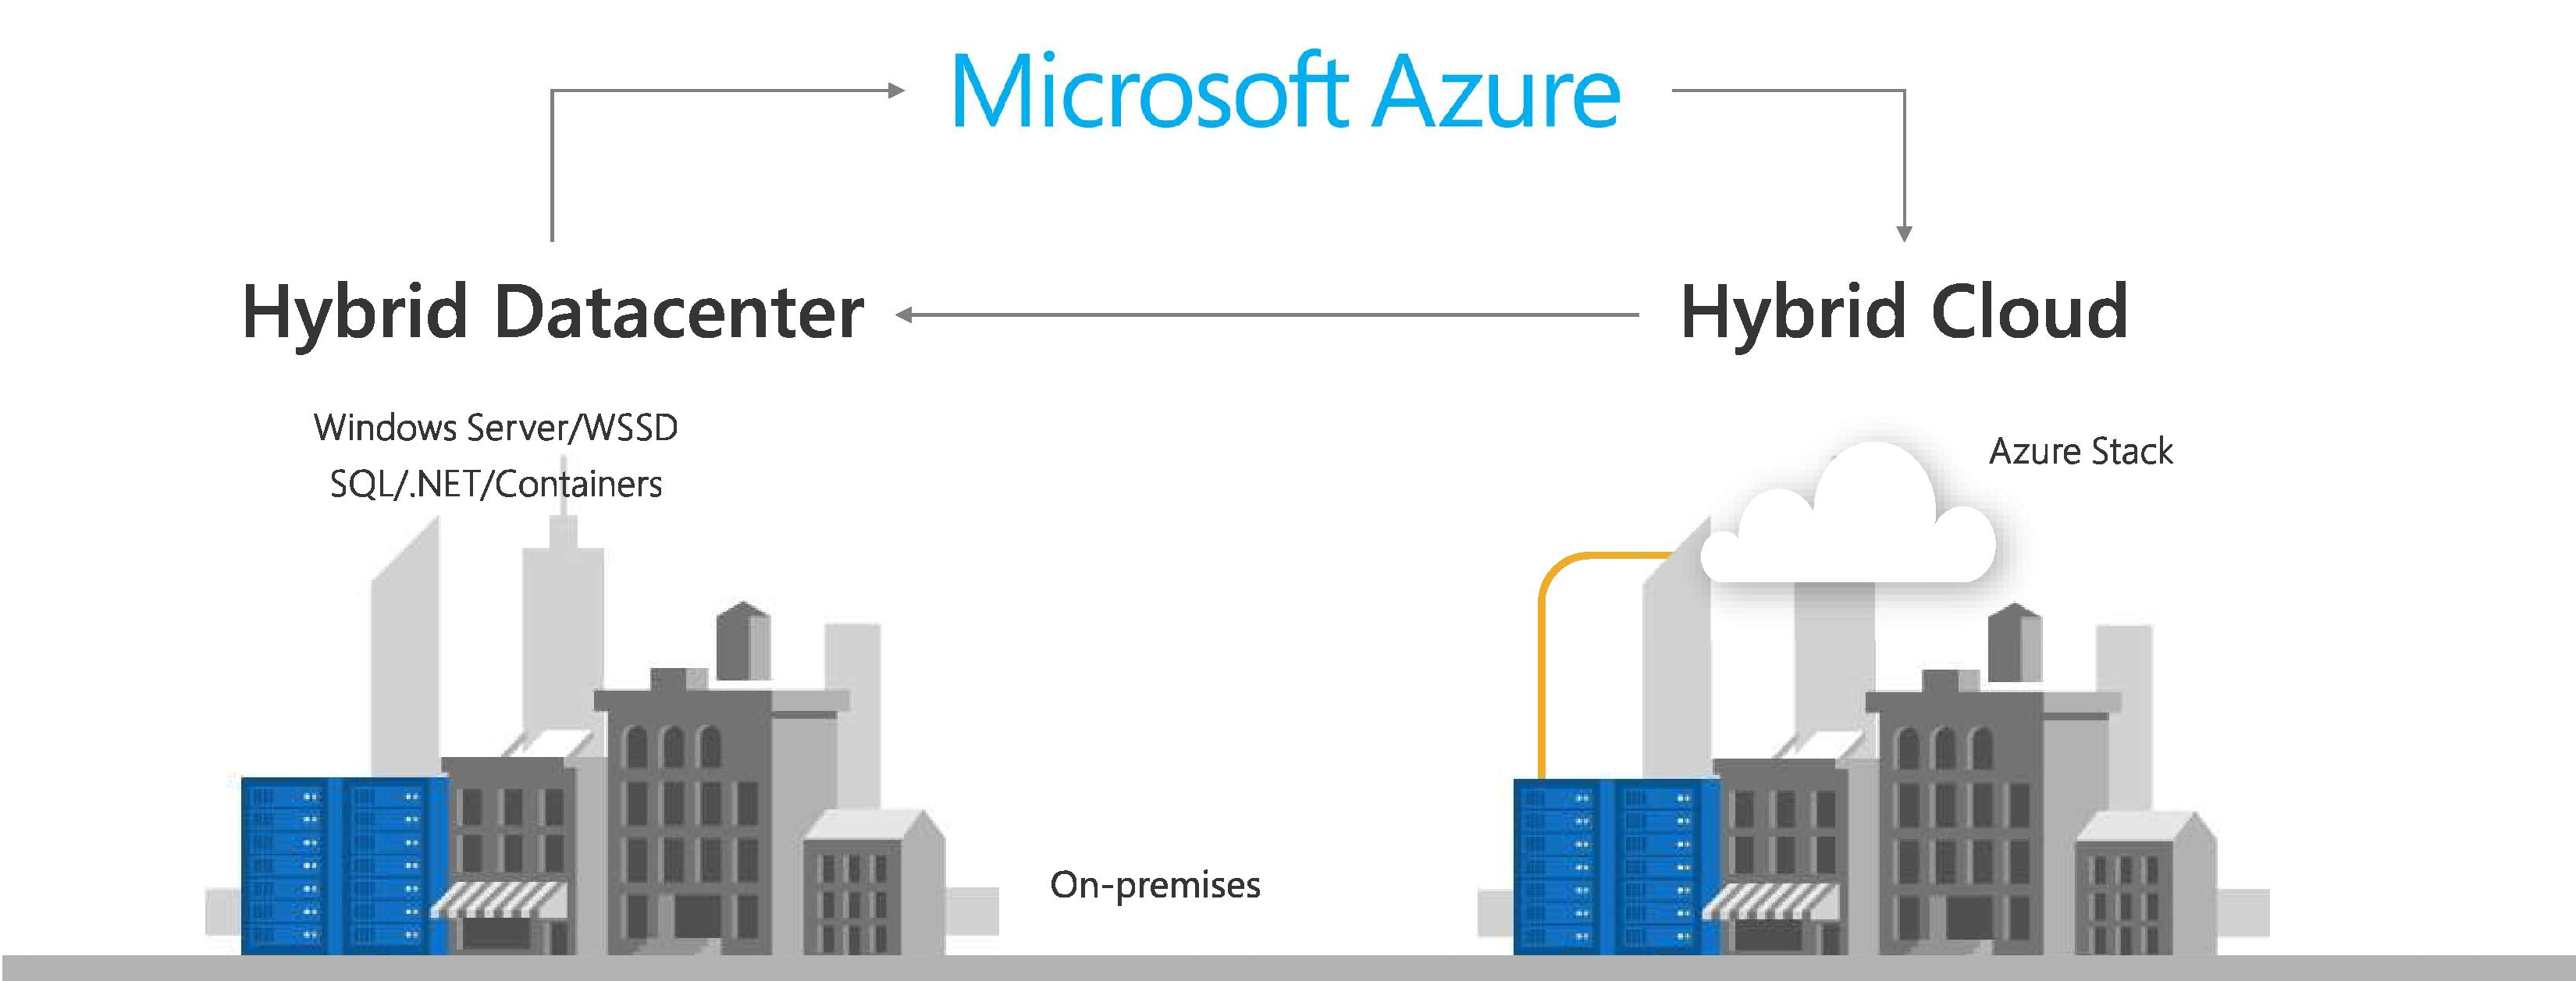
\includegraphics[width=1.0\linewidth]{../bachproef/img/Toekomstvisie/Azure1.png}
    \captionof{figure}{\color{HoGentAccent5} Bridging on-premise and cloud solutions for a modern infrastructure}
\end{center}
\end{multicols}
\end{document}